% Chapter 4

\chapter{Methodology} % Main chapter title

\label{Chapter4} % For referencing the chapter elsewhere, use~\ref{Chapter4} 

In this chapter, we present the methodology of the research. First we present
the threat model in section~\ref{sec:threat-model}.  After that, we show the
overview of ScaRR algorithm to extract checkpoint and list of action in section
\ref{sec:overview}. Section~\ref{sec:scarr-checkpoint-marker} discusses the LLVM
implementation to get checkpoints. Section~\ref{sec:scarr-loa-collector}
discusses on methodology of getting list of actions.  
Checkpoints and list of actions are collected to build offline measurement
database that is used for the remote attestation. The last section shows how to
run the LLVM passes to get the result which is presented in
Chapter~\ref{Chapter5}.

\section{Threat Model}
\label{sec:threat-model}

The threat model in this research is taken from
ScaRR~\cite{toffaliniScaRRScalableRuntime2019}. There are two parties: attacker
and prover. 

\vspace{0.5cm}
\noindent \textbf{Attacker capabilities:} The attacker aims to control remote
service using various method such as memory attack or any attack in user-space.
The attacker has bypassed memory attack protection such as Control Flow
Integrity (CFI) or \( W \bigoplus R \) or ASLR using techniques like
Return-Oriented Programming
(ROP)~\cite{roemerReturnorientedProgrammingSystems2012} or Jump-Oriented
Programming (JOP)~\cite{bletschJumpOrientedProgrammingNew2011}. We do not
consider physical attack and also non-control data attack which does not alter
program's CFG.

\vspace{0.5cm}
\noindent \textbf{Defender capabilities:} The prover uses kernel as trusted
anchor, has common memory corruption attack mitigations such as \( W \bigoplus R
\) and ASLR. Finally, the defender can statically measure the integrity of the
Prover's code (\ie has an hash representation of the Prover's code).


\section{Overview}\
\label{sec:overview}

\begin{figure}[t]
    \centerline{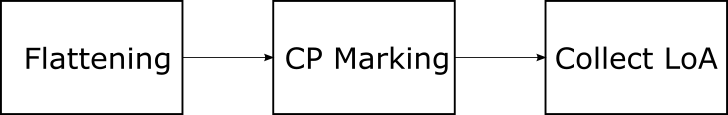
\includegraphics[scale=.70]{Figures/04/scarr-overview.png}}
    \caption{Generating Offline Measurement.}
    \label{fig:scarr-overview}
\end{figure}

The goal of the offline measurement is to get the information to be used in the
remote attestation. In this research we implement ScaRR Control-flow
model~\cite{toffaliniScaRRScalableRuntime2019} which we present in the
Section~\ref{sec:scarr-model}. 

Figure~\ref{fig:scarr-overview} shows the high level step on generating the
offline measurement. First, we inline the source code input (which could be in
an intermediate representation form). Section \ref{sec:code-inlining} describes
the inlining process. Next, we mark the checkpoints from inline code,
particularly marking in the basic block of the code. Section
\ref{sec:scarr-checkpoint-marker} discusses this checkpoint marking step. Last,
for each checkpoint we collect list of actions which indicates how process
traverses to move from one checkpoint to another. Section
\ref{sec:scarr-loa-collector} talks about the process of getting list of
actions.



\section{Code Inlining}
\label{sec:code-inlining}

\begin{listing}[h]
    \inputminted[
    frame=lines,
    framesep=2mm,
    baselinestretch=1.2,
    fontsize=\footnotesize,
    linenos
    ]{c}{Code/04/factorial.c}
    \caption{Program to calculate factorial.}    
    \label{listing:inlining}
\end{listing}

Source code for most applications consist of high level abstraction such as
module, class and function. Programmers write codes in different source files or
also known as translation units for ease of maintenance. In analysing program
control-flow graph, we need to know that the program representation of the
control-flow is correct. Once we compile the program into intermediate
representation, one of high level abstraction that is intact is function.
Function can call another function within the same translation unit or can call
also external function in library. Function can hide additional control-flow in
the function being called. In ScaRR control-flow model, external function call
is one type of checkpoint that needs to be marked. Hence, inlining most internal
function call is important to generate accurate offline measurement. 

Fortunately, inlining is a common optimization process in compiler. In LLVM, we
can use an inlining pass that inlines internal function within the same
translation unit.


Consider a program in listing \ref{listing:inlining}. The main function calls
another internal function. Without inlining, the main function control-flow
graph show no branches and the detail of logic in the factorial function. We
can't generate accurate offline measurement with this original form. However,
after we inline, we can see branches in the control-flow graph which represent
the loop in the code. In this inlined representation we can generate more
accurate offline measurement. Figure \ref{fig:inlining} show the factorial CFG
without inlining and with inlining.


\begin{figure}[h]
    \centerline{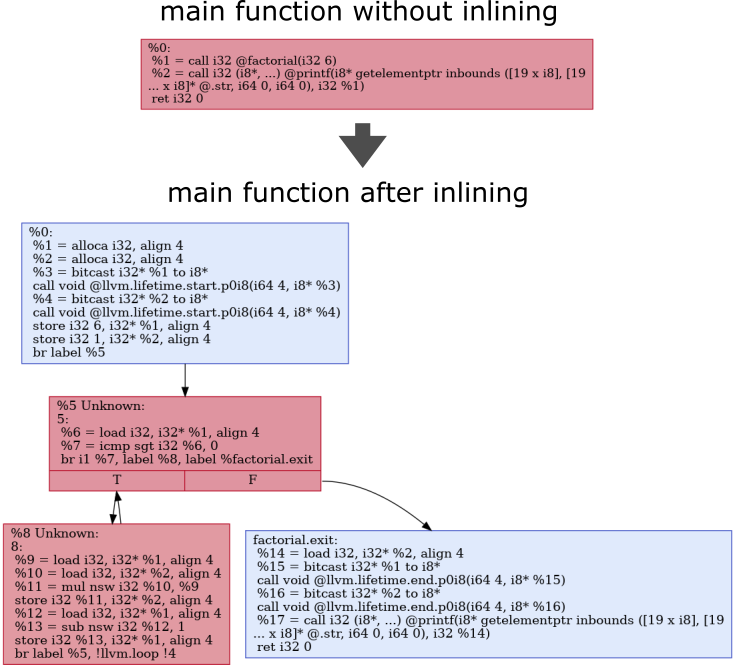
\includegraphics[scale=.80]{Figures/04/inlining-function.png}}
    \caption{Original and Inlined Factorial Program.}
    \label{fig:inlining}
\end{figure}

\section{ScaRR Checkpoint Marker} 
\label{sec:scarr-checkpoint-marker}

Checkpoints and list of actions are used to for offline measurements which is
represented as triplet of first and second checkpoint; and hash of the list of
actions.

$$(cp_A, cp_B, H(LoA)) \Rightarrow [(BBL_{s1}, BBL_{d1}), ..., (BBL_{sn},
BBL_{dn})]$$

The offline measurement is consulted by verifier during remote attestation.

After we inline the code and get program CFG, we will check each of basic block
in CFG to find different kind of checkpoints. In Chapter~\ref{Chapter3} we list
these four types of checkpoints: \textbf{Thread Begin}, \textbf{Thread End},
\textbf{Exit Point} and \textbf{Virtual Checkpoint}. Now we will present the
heuristic on how we will mark as a checkpoint when appropriate.  The logic of
checkpoint marker is to traverse the whole control flow graph at least once. For
each basic block, we have to check whether the basic block can be considered as
any of checkpoint type mentioned above. To allow marking additional information
about ScaRR checkpoint, we are modifying the BasicBlock class to add checkpoint
instance variable as shown in listing~\ref{listing:checkpoint}.

\begin{listing}[htbp]
    \begin{minted}[
        frame=lines,
        framesep=2mm,
        baselinestretch=1.2,
        fontsize=\footnotesize,
        linenos
    ]{c++}
        class BasicBlock ... {
        private:
        // add checkpoint field
            Checkpoint cp;

        public:
            // setter and accessor
        void setCheckpoint(Checkpoint);
        Checkpoint getCheckpoint() const;
        ...
        }
    \end{minted}
    \caption{Add Checkpoint Instance Variable to BasicBlock class.}    
    \label{listing:checkpoint}
\end{listing}

\vspace{0.5cm}
\noindent \textbf{Thread begin} identifies the beginning of a thread or start of
program. In this thesis we mark this checkpoint to first basic block in main
function. If a program is is a multithreaded program, we will mark the thread
begin for each basic block that starts the thread.

\vspace{0.5cm}
\noindent \textbf{Thread end} marks the end of a thread or end of program. In a
multiple-threaded program, we will mark the thread end for each of basic block
that terminates a thread. In this thesis, we mark thread end checkpoint for last
basic block that has no more successors.

\vspace{0.5cm}
\noindent \textbf{Exit point} marks that a basic block is calling function outside of translation
unit. The heuristic of marking this type of basic block is we iterate all
instructions in a basic block. For each instruction, if the instruction is a
\texttt{call} instruction, we check whether the called function has any basic
block. If the function has no basic block, it means it is an external function,
hence we will mark this as an exit point and stop. If none of instruction is a
\texttt{call} instruction or all \texttt{call} instruction in this basic block
call function with non empty basic block, it means this basic block calls
internal function, therefore this basic block is not an exit point. Please refer
to Listing~\ref{listing:exit-point-cp}.

\begin{listing}[htbp]
    \begin{minted}[
        frame=lines,
        framesep=2mm,
        baselinestretch=1.2,
        fontsize=\footnotesize,
        linenos
    ]{c++}
        for (auto &basicBlock: Function) {
            for (auto &instruction : basicBlock) {
                if (isa<CallInst>(i)) {
                auto *call = &cast<CallBase>(i);
                if (call != nullptr && call->getCalledFunction()->empty()) {
                    // this basicBlock is ExitPoint
                    basicBlock.setCheckpoint(Checkpoint::ExitPoint);
                } 
            }
        } 
    \end{minted}
    \caption{Finding ExitPoint Checkpoint}    
    \label{listing:exit-point-cp}
\end{listing}

\vspace{0.5cm}
\noindent \textbf{Virtual checkpoint} is a checkpoint that marks special cases
such as loop or recursion. We will discuss only for loop case in this thesis.
Virtual checkpoint in a loop is basically a loop header. The heuristic to find a
loop header is to use \texttt{DominatorTree} to find a loop. After we find a
loop, then we just need to get the header. Although there is no direct API to
check whether a basic block is a loop header, LLVM provide it in LoopInfoBase
API. See Listing~\ref{listing:virtual-cp}

\begin{listing}[htbp]
    \begin{minted}[
        frame=lines,
        framesep=2mm,
        baselinestretch=1.2,
        fontsize=\footnotesize,
        linenos
    ]{c++}
    void findVirtualCheckpoint(DominatorTree &DT, Function &F) {
        DT.recalculate(F);
        // generate the LoopInfoBase for the current function
        LoopInfoBase<BasicBlock, Loop>* KLoop = new LoopInfoBase<BasicBlock, Loop>();
        KLoop->releaseMemory();
        KLoop->analyze(DT);
        for (auto &bb : F) {
            // Since the BasicBlock would have been inlined, 
            // just traverse from main function
            if (F.getName() == "main") {
                auto loop = KLoop->getLoopFor(&bb);
                if (loop != nullptr) {
                    // found VirtualCheckpoint
                    loop->getHeader()->setCheckpoint(Checkpoint::Virtual);
                }
            }
        }
    }
    \end{minted}
    \caption{Getting Virtual Checkpoint}
    \label{listing:virtual-cp}
\end{listing}




\section{ScaRR LoA Collector}
\label{sec:scarr-loa-collector}

After we mark
checkpoints in the CFG, now we can find list of actions. The step of finding LoA
is traversing path between two checkpoints and add significant basic block that
traverse the path between the two checkpoints. The detail of this step is
explained in section~\ref{sec:scarr-loa-collector}.

\xt{TODO: summarize the algorithm in a pseudocude fashion? you should link the
lines in the pseudo code and describe it step by step.}

\begin{listing}[htbp]
    \begin{minted}[
        frame=lines,
        framesep=2mm,
        baselinestretch=1.2,
        fontsize=\footnotesize,
        linenos
    ]{c++}
    // TBD
    \end{minted}
    \caption{TBD Pseudocode for LoA}
    \label{listing:loa-pseudocode}
\end{listing}

The algorithm of getting LoA between two checkpoints is little bit more complex.
First, we iterate all the basic block and if the basic block is a checkpoint we
mark this is $cpA$. Next, we recursively traverse the successor of $cpA$ until
we find another checkpoint $cpB$. It is possible for $cpA = cpB$. If there is no
branch between the two checkpoint, the LoA is an empty set. If there is a
branch, the first LoA is always be $cpA$ and the second LoA is always be the
first basic block after the branch \textemdash{} which can be $cpB$ or just non
checkpoint basic block. Interested readers can refer to the implementation of
this pass to see the detail.
